\chapter{Experimental Setup} \label{chap:exp_setup}

\section{Vortex Configuration}

\textcolor{red}{This is wrong, now using RTLSIM to save simulation time, results are close to equal}

The Vortex project has a built-in script for running benchmarks. The scripts allows for setting several parameters and configurations for the benchmarks, architecture and simulator. \Gls{vortex}' simulation stack includes four simulation environments. My setup utilize \textit{VLSIM}. VLSIM use Verilator \cite{verilator} to simulate the full RTL design and implements the accelerator functional unit (AFU) interface in software, as well as simulating memory using Ramulator \cite{Ramulator}. The configurations I used are listed in Table \ref{tab:vortex_config}, while the benchmarks are listed in Table \ref{tab:benchmarks}. In my project thesis \cite{Aurud_Project}, I tested a range of configurations with different number of cores. I found that for up to 32 cores all benchmarks worked as intended, while for 64 cores some of the benchmarks failed. This is why I elected to continue evaluating Vortex with 32 cores.

% -- Table of Vortex Configurations
\begin{table}
    \centering
    \caption{Configurations for the Vortex architecture.}
    \begin{tabular}{|l|l|} 
    \hline
    \multicolumn{2}{|c|}{\textbf{Vortex Configuration}} \\ \hline
     
    \makecell[l]{GPU cores} & \makecell[l]{32 cores, 1.2GHz, 16 threads/core, \\ 4 threads/warp, 4 warps/core} \\ \hline

    \makecell[l]{Clustering} & \makecell[l]{8 cores/cluster} \\ \hline
     
    \makecell[l]{GPU L1 Cache} & \makecell[l]{16KiB per core, direct mapped, \\ 16B blocks, 4B words} \\ \hline

    \makecell[l]{GPU L2 Cache} & \makecell[l]{128KiB per cluster, direct mapped \\ 64B blocks} \\ \hline

    \makecell[l]{DDR4} & \makecell[l]{DDR4 2400R (1200 MHz), 19.2GB/s, \\ 4Gbx8, 1 channel, 1 rank/channel \\ $t_{CL}=16$, $t_{RCD}=16$, $t_{RP}=16$} \\ \hline
     
    NoC & Hierarchical tree structure \\ \hline
    \end{tabular}
    \label{tab:vortex_config}
\end{table}

% -- Table of benchmarks
\begin{table}
    \centering
    \caption{Overview of benchmarks and the adjusted input sizes}
    \begin{tabular}{|l|l|l|l|} 
        \hline
        \makecell[l]{\textbf{Benchmark}}         & \makecell[l]{\textbf{Name}} & \makecell[l]{\textbf{Default} \\ \textbf{Input Size}}    & \makecell[l]{\textbf{Adjusted} \\ \textbf{Input Sizes}} \\ \hhline{|=|=|=|=|}
        Vector Addition            & vecadd        & 64                             & 32768              \\ \hline
        General Matrix Multiply    & sgemm         & 32x32 Matrix                   & 256x256 Matrix          \\ \hline
        Matrix Filter (3x3 kernel) & sfilter       & 16                             & 1024         \\ \hline
        Sorting                    & psort         & 16                             & 8192  \\ \hline
        A times X plus Y           & saxpy         & 16                             & 262144 ($2^{18}$)  \\ \hline
        Nearest Neighbour Search   & nearn         & 40k Records                    & - \\ \hline
        B+ Tree Graph Traversal    & b+tree        & 1M Elements                    & 10K Elements \\ \hline
        Back propogation           & backprop      & 65536                          & - \\ \hline
        Gaussian elimination       & gaussian      & 16x16 Matrix                   & 512x512 Matrix \\ \hline
        Heart Wall                 & hw     & 20 Frames                      & - \\ \hline
        HotSpot                    & hotspot       & 512 2 2                        & 512 2 2  \\ \hline
        HotSpot3D                  & 3D     & 512 8 100                      & 512 8 4  \\ \hline
        LavaMD2                    & lavaMD        & -boxes1d 10                    & -boxes1d 16 \\ \hline
        SRAD                       & srad          & 502x458 Image                  & 251x229 Image  \\ \hline
        Streamcluster              & sc            & 65536 Points                   & - \\ \hline
        Breadth-First Search       & bfs & 4096 Nodes                               & 65536 Nodes  \\ \hline
        CFD Solver                 & cfd & fvcorr.domn.097K                 & missile.domn.0.2M  \\ \hline
        LU Decomposition           & lud & 1024x1024 Matrix                         & -  \\ \hline
        GPUDWT                     & dwt2d & 192x192 Bitmap                         & -  \\ \hline
        \makecell[l]{Kmeans}                     & \makecell[l]{kmeans} & \makecell[l]{100 Points,\\100 Features}       & \makecell[l]{2048 Points \\ 128 Features} \\ \hline
        \makecell[l]{Needleman-Wunsch}           & \makecell[l]{nw}            & \makecell[l]{2048x2048 Matrix \\ 10 Penalty}     & \makecell[l]{-}  \\ \hline
    \end{tabular}
    \label{tab:benchmarks}
\end{table}

\section{Benchmarks}
\textcolor{red}{Rewrite section after writing about the methods an earlier chapter}
In my project thesis \cite{Aurud_Project}, I found that the benchmarks included by \Gls{vortex} required a much larger input size than default, to give reasonable performance results. I.e having realistic memory usage and no idling cores. The adjusted input sizes as well as the inputs for the new benchmarks are displayed in Table \ref{tab:benchmarks}.

Software simulation is much slower than running on ASICs or FPGAs. To keep the simulation time reasonable, I implement fast-forwarding, warm-up and early termination. \textit{Early termination} is implemented such that when \Gls{vortex} has ran for a given number of cycles, it jumps to the exit routine and dumps all performance metrics. This allows us to run benchmarks with realistic working-sets, to obtain realistic performance metrics. It is not ideal to terminate early, as the full behaviour of the benchmarks might not be captured. Additionally will changes to the architecture change the number of instructions executed within the simulated cycles. This is still a common solution \cite{simpoint}, as there are not many other options. Due to the increased number of benchmarks it is still likely that the results will be representable of \Gls{vortex}' performance.  


% It would be ideal to terminate based on the number of instructions committed, such that benchmark behaviour would be independent of changes to performance. However, as each core terminate based on internal metrics, cores with idle warps, would commit less instructions, using a disproportionate number of cycles compared to a core full of active warps. Thus I decided to terminate early based on cycle count.

\textit{Fast-forwarding} is done by not collecting performance metrics in the start of the simulation. When doing early termination, the start of the simulation (e.g starting warps) represents a larger proportion of the total run-time. Not including the start-up, is thus important to obtain performance metrics representing the majority of the runtime. \textit{Warm-up} is removing the cold-start bias occurring at the beginning of the benchmark. This is due to empty caches, branch buffers, pre-fetchers, etc. By extending the number of cycles fast-forwarded, the GPU can be warmed up to give a more stable performance when simulating less cycles.

Initially the L1 and L2 cache hit-rates were collected for a subset of the benchmarks. These are plotted in \ref{fig:l1_cache_hitrate} and \ref{fig:l2_cache_hitrate} for L1 and L2 cache respectively. After 30000 cycles, the cache hit-rate is stabilizing for both the L1 and L2 cache. While the L1 hit-rate for backprop is fluctuating, this is probably due to its access pattern, as similar fluctuations show up. To give some extra margins, 50000 was selected as the number of cycles to fast-forward.

For benchmarks with multiple kernels, the start-up time of each kernel become a relevant if the benchmark is not exited by early part of the performance...

\begin{figure}
    \centering
    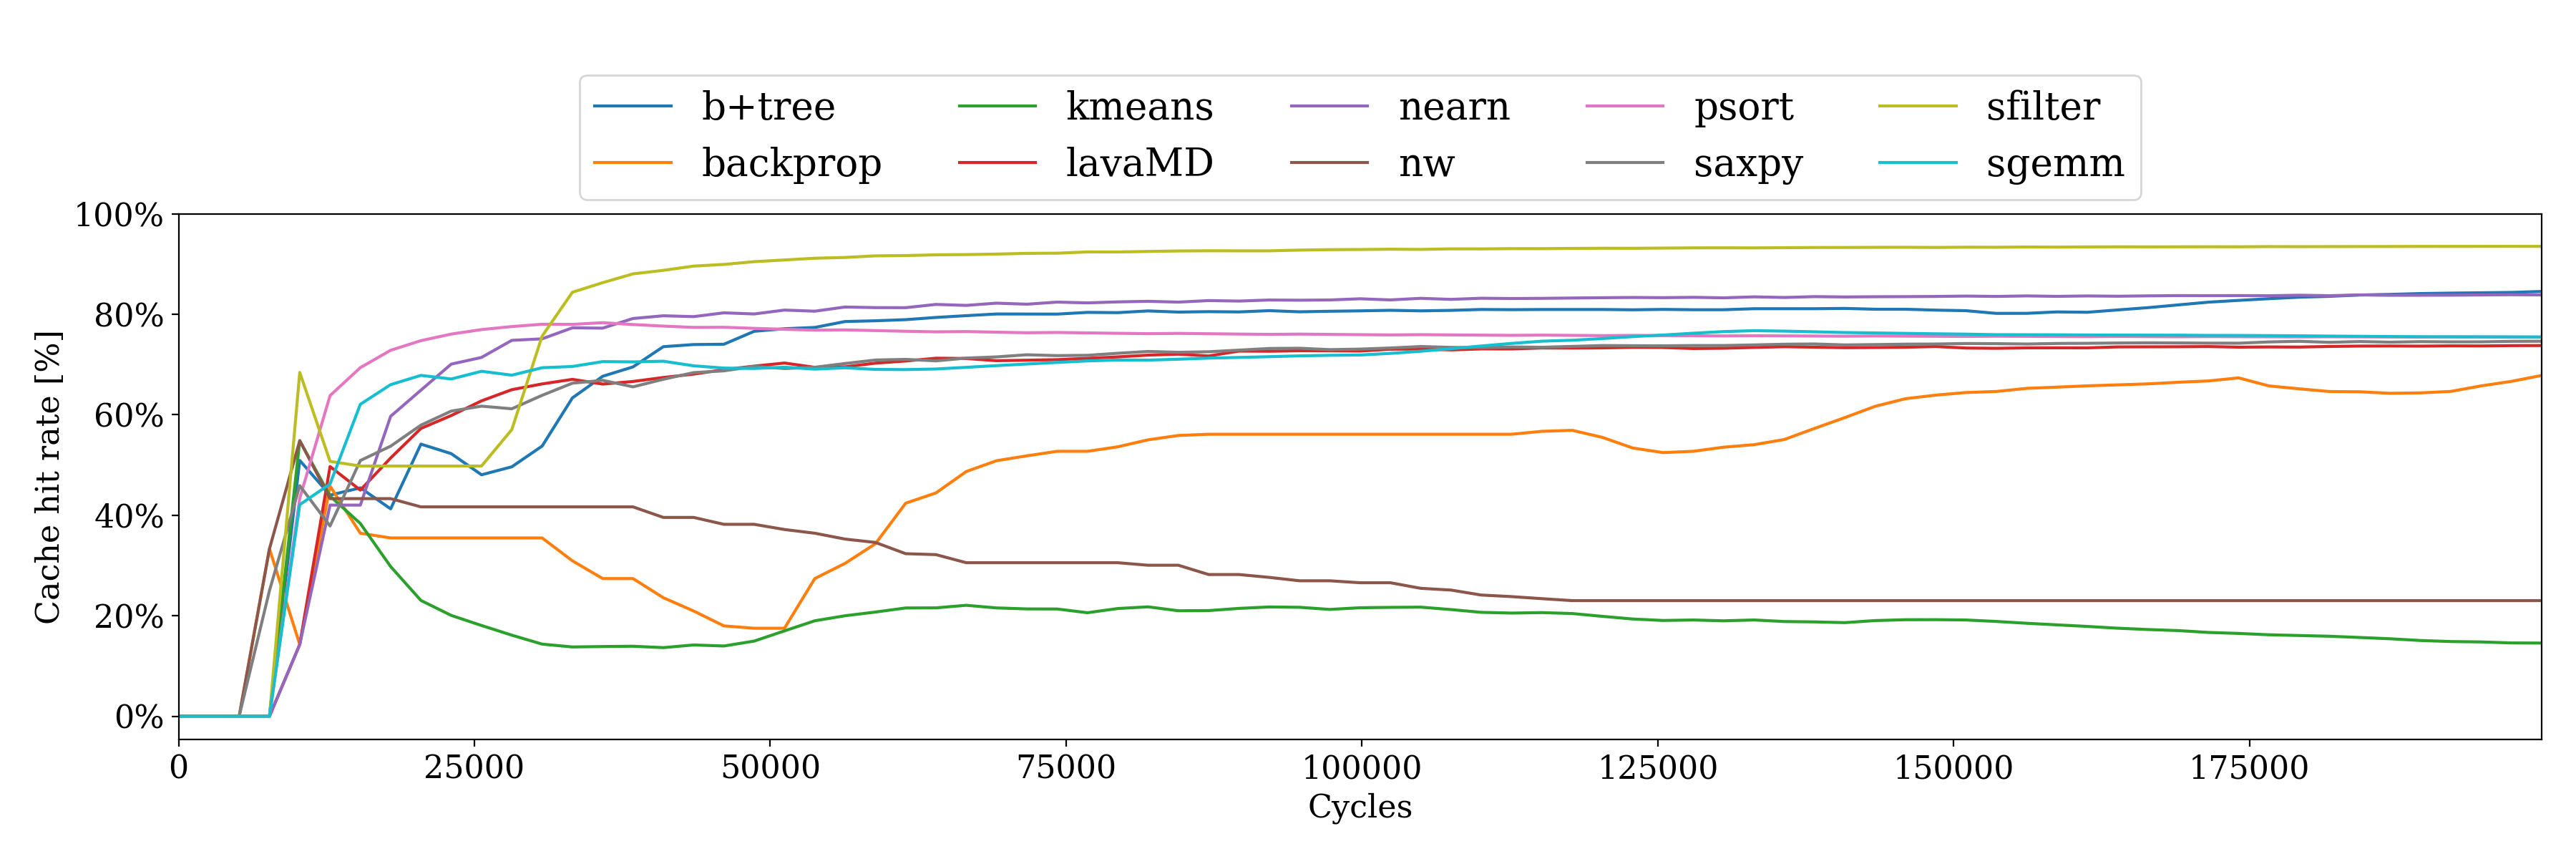
\includegraphics[width=\textwidth]{figures/L1cachehit_vlsim.png}
    \caption{L1 dcache hit rate during startup}
    \label{fig:l1_cache_hitrate}
\end{figure}


\begin{figure}
    \centering
    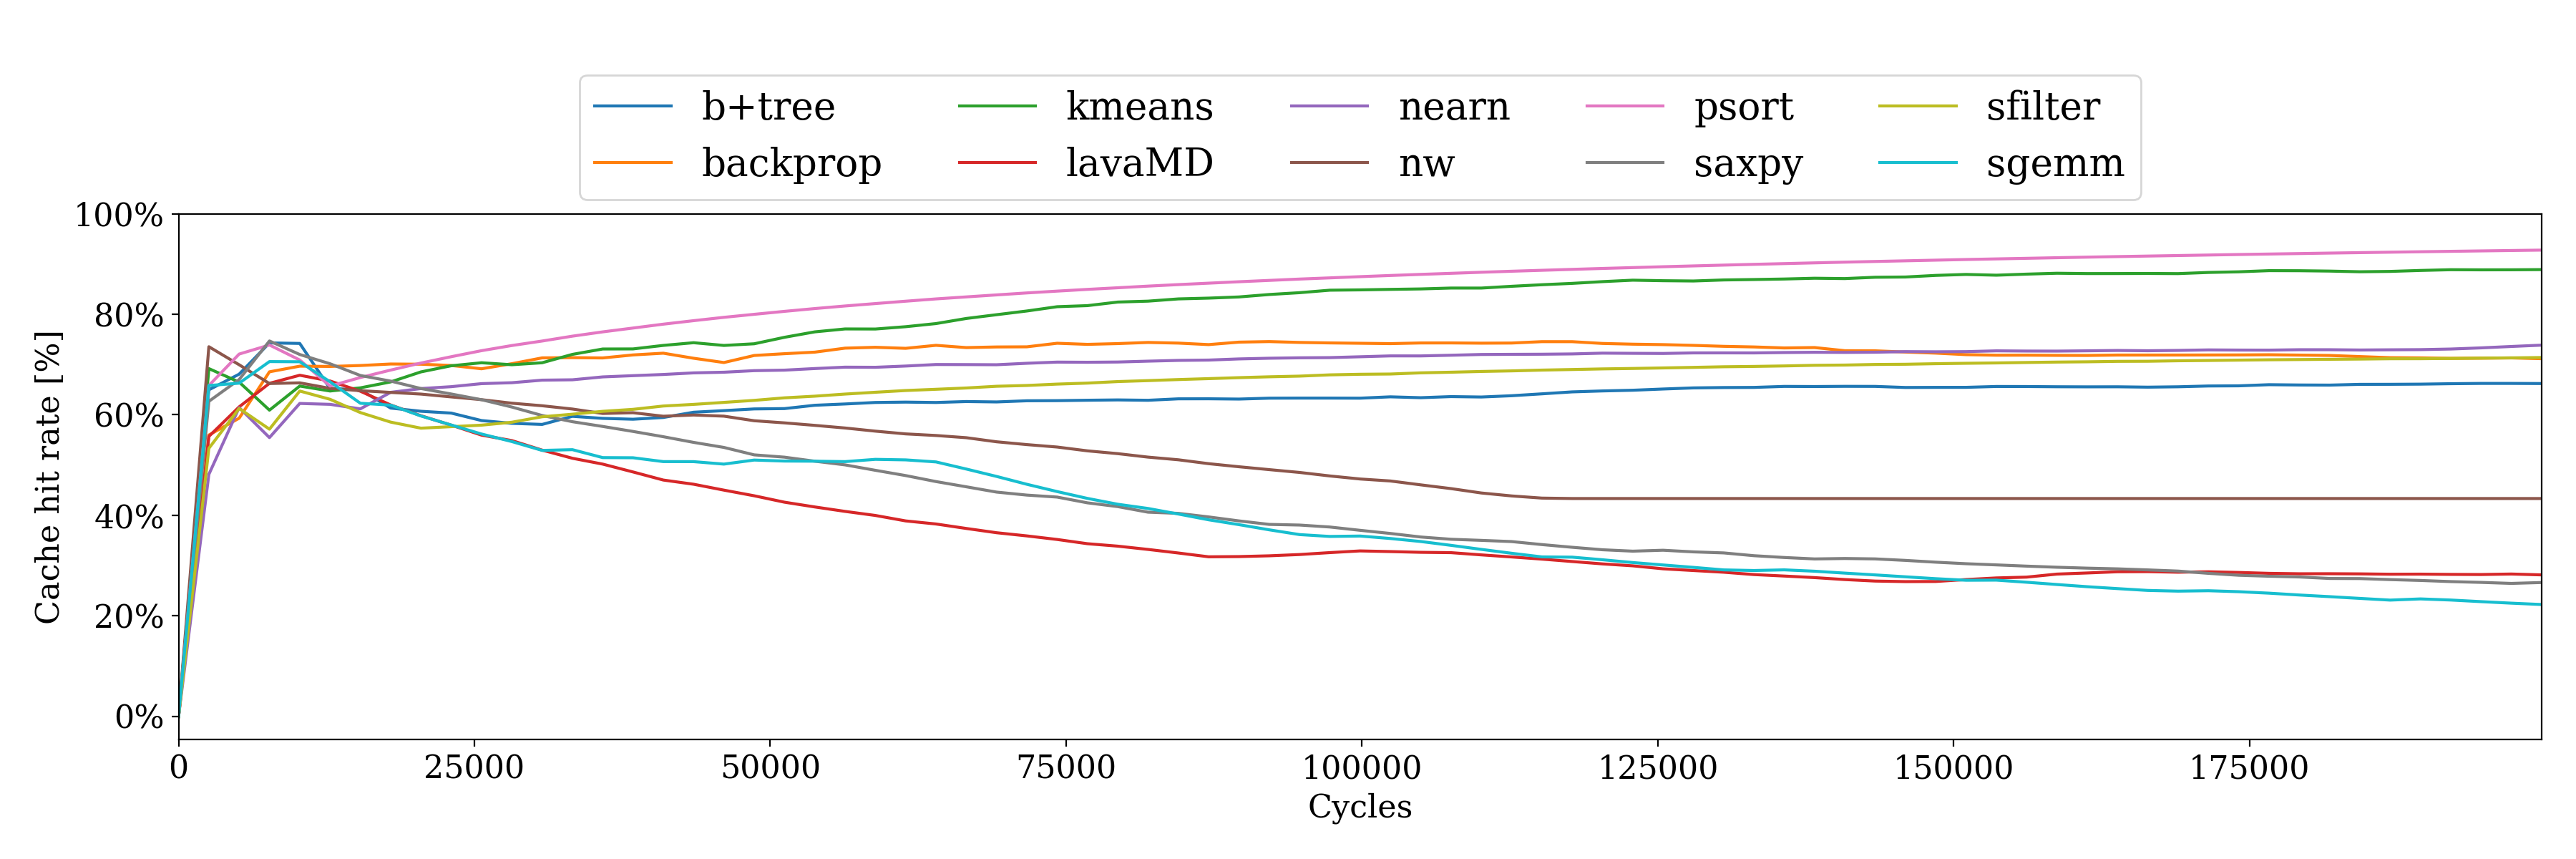
\includegraphics[width=\textwidth]{figures/L2cachehit_vlsim.png}
    \caption{L2 dcache hit rate during startup}
    \label{fig:l2_cache_hitrate}
\end{figure}

\section{IDUN Cluster}

All the simulations were ran on the IDUN Cluster \cite{Idun_tech_report}. When running the benchmarks with the adjusted input sizes, each benchmark require substantial time to complete. Using IDUN allowed us to run all benchmarks in parallel. This saved a lot of time, as some of the benchmarks required multiple hours to complete.

The installation of vortex had to be modified due to missing permissions to write to some of the install locations. It also followed that the locations of these dependencies had to be changed in the Vortex makefiles.